\section{The group $\Gamma_1(5)$}

The fundamental domain of the group $\Gamma_1(5) = \{ (\begin{smallmatrix}
    a & b \\ c & d
\end{smallmatrix}) \in \SL_2(\bZ): a \equiv d \equiv 1 \pmod{5}, c \equiv 0\pmod{5}\}$ can be pictured as below.
The cusps are given by $0, \frac{1}{2}, \frac{2}{5}, i\infty$.
\begin{center}
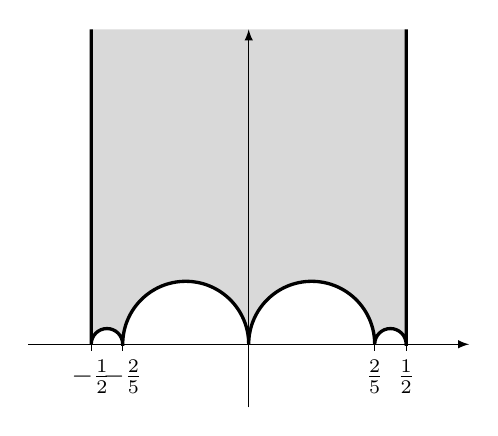
\begin{tikzpicture}[scale=4]
    \draw[very thick, fill=gray!30]
        (-.5,1) -- (-.5,0) --
        (-1/2, 0) arc (180:0:1/20) --
        (-2/5, 0) arc (180:0:1/5) --
        (0, 0) arc (180:0:1/5) --
        (2/5, 0) arc (180:0:1/20) --
        (.5, 0) -- (.5,1);
    \draw[-latex] (-0.7,0) -- (0.7,0);
    \draw[-latex] (0,-.2) -- (0,1);
    \draw(-.5,.02)--(-.5,-.02)node[below]{$-\frac{1}{2}$};
    \draw(.5,.02)--(.5,-.02)node[below]{$\frac{1}{2}$};
    \draw(-2/5,.02)--(-2/5,-.02)node[below]{$-\frac{2}{5}$};
    \draw(2/5,.02)--(2/5,-.02)node[below]{$\frac{2}{5}$};
\end{tikzpicture}
\end{center}
They are regular and have widths $5, 5, 1, 1$ respectively.
Consider the following function,
$$
y(\tau) = q \prod_{n = 1}^{\infty} (1 - q^n)^{5 \left(\frac{n}{5}\right)}
$$
where $\left(\frac{n}{5} \right)$ it the Legendre symbol.
The function $y(\tau)$ is a hauptmodul for the group $\Gamma_1(5)$.
Moreover, $y(0) = - \frac{11}{2} + \frac{5}{2} \sqrt{5}, y(\frac{2}{5}) = i\infty, y(\frac{1}{2}) = -\frac{11}{2} - \frac{5}{2} \sqrt{5}, y(i\infty) = 0$.
The function $y(-\frac{1}{5\tau})$ is again modular with respect to $\Gamma_1(5)$ and one easily checks that
$$
y\left(-\frac{1}{5 \tau}\right) = \frac{\lambda_1 - y(\tau)}{1 + \lambda_1 y(\tau)}, \quad \lambda_1 = -\frac{11}{2} + \frac{5}{2} \sqrt{5}.
$$
So the function
$$
    t(\tau) = y(\tau) \frac{\lambda_1 - y(\tau)}{1 + \lambda_1 y(\tau)}
$$
is invariant under the involution $t \mapsto -1 / 5\tau$.
In a similar way as in Proposition \ref{prop:2.1} one shows,

\begin{proposition}
\label{prop:3.1}
The function $t(\tau)$ maps the shaded open area in the picture below univalently onto the upper half plane and satisfies
$$
    t(i\infty) = 0, \quad t\left(\frac{i}{\sqrt{5}}\right) = (\lambda_2 + \sqrt{1 + \lambda_2^2})^2, \quad t \left(\frac{4}{9} + \frac{i}{9\sqrt{5}}\right) = (\lambda_2 - \sqrt{1 + \lambda_2^2})^2, \quad t\left(\frac{1}{2}\right) = \infty
$$
where $\lambda_2 = \frac{11}{2} - \frac{5}{2} \sqrt{5}$.
\end{proposition}

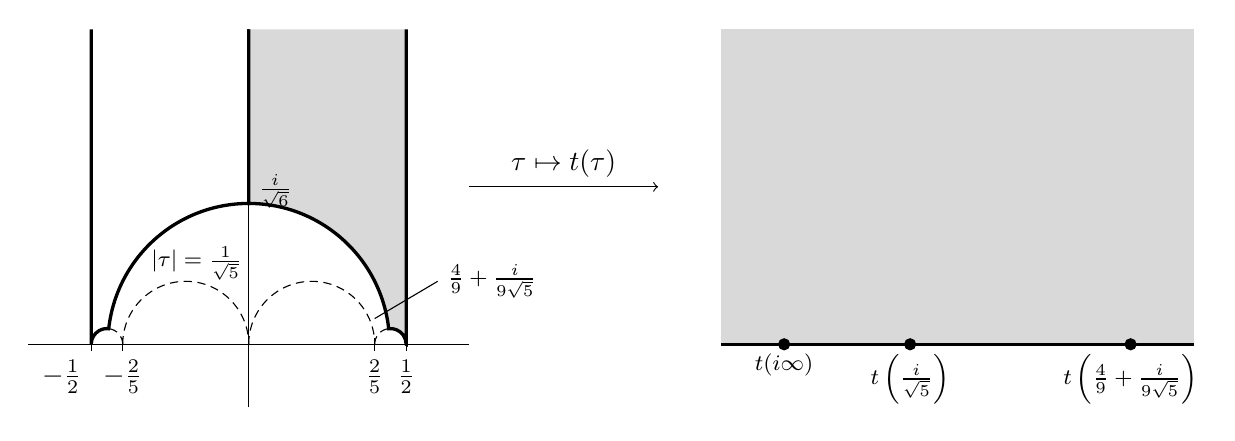
\begin{tikzpicture}[scale=4]
    \draw[very thick]
        (-.5,1) -- (-.5,0) --
        (-1/2, 0) arc (180:78.5:1/20) --
        (-4/9, {1/(9 * sqrt(5))}) arc (173.62:90:{1/sqrt(5)}) --
        (0,{1/sqrt(5)}) -- (0,1);
    \draw[very thick, fill=gray!30]
        (0,1) --
        (0, {1/sqrt(5)}) arc (90:6.38:{1/sqrt(5)}) --
        (4/9, {1/(9 * sqrt(5))}) arc (96.38:0:1/20) --
        (1/2,0) -- (1/2,1);
    \draw (-0.7,0) -- (0.7,0);
    \draw (0,-.2) -- (0,1);
    \draw (0,0.4)node[above right, font=\footnotesize]{$\frac{i}{\sqrt{6}}$};
    \draw[densely dashed] (-2/5, 0) arc (0:83.62:1/20);
    \draw[densely dashed] (-2/5,0) arc (180:0:1/5);
    \draw[densely dashed] (2/5,0) arc (180:96.38:1/20);
    \draw[densely dashed] (0,0) arc (180:0:1/5);
    \draw(-.5,.02)--(-.5,-.02)node[below left]{$-\frac{1}{2}$};
    \draw(.5,.02)--(.5,-.02)node[below]{$\frac{1}{2}$};
    \draw(-2/5,.02)--(-2/5,-.02)node[below]{$-\frac{2}{5}$};
    \draw(2/5,.02)--(2/5,-.02)node[below]{$\frac{2}{5}$};
    \draw (2/5, {1/(5 * sqrt(6))}) -- (0.6,0.2)node[right, font=\footnotesize]{$\frac{4}{9} + \frac{i}{9\sqrt{5}}$};
    % \draw (-0.25, 0.5)node[above]{II};
    % \draw (0.25, 0.5)node[above]{I};
    \draw (-0.34, 0.34)node[below right, font=\footnotesize]{$|\tau| = \frac{1}{\sqrt{5}}$};

    \draw[->] (0.7,0.5) -- (1.3,0.5);
    \draw (1.0, 0.5)node[above]{$\tau \mapsto t(\tau)$};

    \fill[gray!30] (1.5,1.0) -- (1.5,0) -- (3.0, 0) -- (3.0, 1.0);
    \draw[very thick] (1.5,0) -- (3,0);
    \draw[fill] (1.7,0) circle (0.5pt)node[below, font=\footnotesize]{$t(i\infty)$};
    \draw[fill] (2.1,0) circle (0.5pt)node[below, font=\footnotesize]{$t\left(\frac{i}{\sqrt{5}}\right)$};
    \draw[fill] (2.8,0) circle (0.5pt)node[below, font=\footnotesize]{$t\left(\frac{4}{9}+\frac{i}{9\sqrt{5}}\right)$};
\end{tikzpicture}

We also consider the function
$$
    s(\tau) = y(\tau) \frac{\lambda_2 - y(\tau)}{1 + \lambda_2 y(\tau)}, \quad \lambda_2 = \frac{11}{2} - \frac{5}{2} \sqrt{5}.
$$

\begin{lemma}
    \label{lem:3.2}
    The branching values of $s(\tau)$, as defined in Section 1, read $0, \infty$ and $(\lambda_1 \pm \sqrt{1 + \lambda_1^2})^2$ where $\lambda_1 = -\frac{11}{2} + \frac{5}{2} \sqrt{5}$.
\end{lemma}

\begin{proof}
    The branching values of $s(\tau)$ are the values of $s(\tau)$ at the cusps or the values at the points $\tau$, $\Im \tau > 0$ where $s'(\tau) = 0$.
    The values at the cusps are $0, \infty$.
    Notice that
    $$
        \frac{s'}{s} = \left(1 + \frac{y}{y - \lambda_2} - \frac{y}{y - \lambda_1}\right) \frac{y'}{y} = \frac{y^2 + (11 - 5\sqrt{5})y - 1}{y^2 + 11 y - 1} \frac{y'}{y}.
    $$
    The function $\frac{y'}{y}$ can only be zero at the cusps $0, \frac{1}{2}$.
    If $y^2 + (11 - 5\sqrt{5})y - 1 = 0$ then $y = \lambda_1 \pm \sqrt{1 + \lambda_1^2}$ which implies $s = (\lambda_1 \pm \sqrt{1 + \lambda_1^2})^2$.
\end{proof}

Notice that the $q$-expansions of $t(\tau)$, $s(\tau)$ read
$$
    t(\tau) = \sum_{n=1}^{\infty} a_n q^n, \quad s(\tau) = \sum_{n=1}^{\infty} b_n q^n
$$
where $a_n, b_n$ are algebraic integers in $\bQ(\sqrt{5})$.
From the construction follows that for every $n$ the numbers $a_n, b_n$ are conjugates.

\begin{theorem}
    \label{thm:4}
    Let $L(3, \chi) = \sum_{n=1}^{\infty} \left(\frac{n}{5}\right) n^{-3}$, where $\left(\frac{n}{5}\right)$ is the Legendre symbol.
    Then $8\zeta(3) - 5\sqrt{5}L(3, \chi)$ is not in $\bQ(\sqrt{5})$.
\end{theorem}

\begin{proof}
    Consider the weight 4 form on $\Gamma_1(5)$ given by
    $$
        24 F(\tau) = E_4(\tau) - 25 E_4(5\tau) + 24(E_4(\chi, \tau) - 5\sqrt{5} F_4(\chi, \tau))
    $$
    where
    \begin{align*}
        E_4(\chi, \tau) &= 1 + \sum_{n=1}^{\infty} \left(\frac{n}{5}\right) \frac{n^3 q^n}{1 - q^n}, \\
        F_4(\chi, \tau) &= \sum_{m, n=1}^{\infty} \left(\frac{n}{5}\right) m^3  q^{mn}.
    \end{align*}
    Note that up to a constant factor, $F(\tau)$ is cahracterised by the facts $F(\tau) \in \rM_4(\Gamma_1(5))$, $F(i\infty) = 0$, $F(-\frac{1}{5\tau}) = -25 \tau^4 F(\tau)$.
    The corresponding Dirichlet series reads
    $$
        L(F, s) = 10 (1 - 5^{2-s})\zeta(s) \zeta(s - 3) + \zeta(s) L(s - 3, \chi) - 5\sqrt{5} \zeta(s - 3) L(s, \chi)
    $$
    where
    $$
        L(s, \chi) = \sum_{n=1}^{\infty} \left(\frac{n}{5}\right) n^{-s}.
    $$
    Define $f(\tau)$ by $f(i\infty) = 0$, $(\frac{\dd}{\dd \tau})^{3} f(\tau) = (2\pi i)^3 F(\tau)$.
    then, from Proposition \ref{prop:1.2} follows that
    $$
        5 \tau^2 \left(f\left(-\frac{1}{5\tau}\right) - A\right) = - (f(\tau) - A)
    $$
    where
    \begin{align*}
        A &= 10\left(1 - \frac{1}{5}\right) \zeta(3) \zeta(0) + \zeta(3) L(0, \chi) - 5\sqrt{5} \zeta(0) L(3, \chi) \\
        &= -\frac{1}{3} (8\zeta(3) - 5\sqrt{5} L(3, \chi)).
    \end{align*}
    Now let 
    $$
        -8 E(\tau) = E_2(\tau) - 5 E_2(5\tau) + 20 (E_2(\chi, \tau) - \sqrt{5} F_2(\chi, \tau))
    $$
    where
    \begin{align*}
        E_2(\chi, \tau) &= -\frac{1}{5} + \sum_{n=1}^{\infty} \left(\frac{n}{5}\right) \frac{n q^n}{1 - q^n}, \\
        F_2(\chi, \tau) &= \sum_{m, n=1}^{\infty} \left(\frac{n}{5}\right) m q^{mn}.
    \end{align*}
    The function $E(\tau)$ satisfies $E(-\frac{1}{5\tau}) = -5\tau^2 E(\tau)$, hence $E(\tau) (f(\tau) - A)$ is fixed under the involution $\tau \mapsto -1/5\tau$.
    Consider $E(\tau)$ and $E(\tau)f(\tau)$ as functions of $t = t(\tau)$ and write
    $$
        E(\tau)f(\tau) = \sum_{n=1}^{\infty} c_n q^n, \quad E(\tau) = \sum_{n=1}^{\infty} d_n q^n.
    $$
    By construction it follows that $d_n$ and $[1, \dots, n]^3 c_n$ are algebraic integers in $\bQ(\sqrt{5})$.
    Just as in the proof of Theorem \ref{thm:1}, we observe that the radius of convergence of $E(t)(f(t) - A)$ equals $(\lambda_2 + \sqrt{1 + \lambda_2^2})^2$\footnote{There's a typo in the original article: sign is fixed.} and hence for all $\epsilon > 0$,
    \begin{equation}
        \label{eqn:5}
        |c_n - A d_n| < (\lambda_2 + \sqrt{1 + \lambda_2^2})^{(2 - \epsilon)n} \quad \forall n > n_0(\epsilon).
    \end{equation}
    Now consider the functions
    $$
        24 \overline{F}(\tau) = E_4(\tau) - 25 E_4(5\tau) + 24(E_4(\chi, \tau) + 5\sqrt{5} F_4(\chi, \tau)) 
    $$
    the corresponding third primitive $\overline{f}(\tau)$ and
    $$
        -8 \overline{E}(\tau) = E_2(\tau) - 5 E_2(5\tau) + 20 (E_2(\chi, \tau) + \sqrt{5} F_2(\chi, \tau)).
    $$
    Consider them as functions of $s = s(\tau)$ and write
    $$
        \overline{E}(\tau) \overline{f}(\tau) = \sum_{n=1}^{\infty} \overline{c}_n q^n, \quad \overline{E}(\tau) = \sum_{n=1}^{\infty} \overline{d}_n q^n.
    $$
    From the construction follows that $\overline{c}_n, \overline{d}_n$ are conjugates of $c_n, d_n$ respectively.
    By Lemma \ref{lem:3.2} the smallest nonzero branching value of $s(\tau)$ equals $(-\lambda_1 + \sqrt{1 + \lambda_1^2})^{2}$ and hence the radius of convergence of both $\sum_{n=1}^{\infty} \overline{c}_{n} s^n$ and $\sum_{n=1}^{\infty} \overline{d}_{n} s^n$ is at least $(-\lambda_1 + \sqrt{1 + \lambda_1^2})^{2}$.
    Hence for any $\theta \in \bC$ and any $\epsilon > 0$
    \begin{equation}
        \label{eqn:6}
        |\overline{c}_n - \theta \overline{d}_n| < (\lambda_1 + \sqrt{1 + \lambda_1^2})^{(2 + \epsilon) n} \quad \forall n > n_1(\epsilon, \theta).
    \end{equation}
    Now suppose $A \not\in \bQ(\sqrt{5})$.
    Let $\overline{A}$ be its conjugate and let $d$ be its denominator.
    Multiplication of \eqref{eqn:5} and \eqref{eqn:6} with $\theta = \overline{A}$ yields
    \begin{equation}
        \label{eqn:7}
        |c_n \overline{c}_n - (c_n \overline{d}_n \overline{A} + \overline{c}_n d_n A) + d_n \overline{d}_n A\overline{A}| < \left(\frac{1}{20.3}\right)^{2n} \quad \forall n > n_0.
    \end{equation}
    Since $c_n \overline{c}_n \in \bZ / [1, \dots, n]^{6}$, $c_n \overline{D}_n \overline{A} + \overline{c}_n d_n A \in \bZ / d[1, \dots, n]^{3}$, $d_n \overline{d}_n A \overline{A} \in \bZ / d^2$ and $d^2 [1, \dots, n]^6 < (20.1)^{2n} < (20.3)^{2n}$ for sufficiently large $n$.
    Hence $c_n - d_n A = 0$ for $n$ large enough, and we have a contradiction.
    Theorem \ref{thm:4} now follows.
\end{proof}

\begin{remark*}
By some tedius calculation one can veritfy that the numbers $d_n$ satisfy the recurrence relation 
\begin{align*}
    (n + 1)^{3} d_{n+1} &= ((124 + 55\sqrt{5})n(n+1) + 34 + 15\sqrt{5}) (2n + 1)d_n - n^3 d_{n-1} \\
    d_0 = 1, d_1 &= 34 + 15\sqrt{5}, d_2 = 7111 + 3180 \sqrt{5}, d_3 = 2040334 + 912465\sqrt{5}.
\end{align*}
\end{remark*}

\begin{theorem}
    \label{thm:5}
    The number $\zeta(2) = \frac{\pi^2}{6}$ is irrational.
    \end{theorem}
\begin{proof}
    Consider the function
    $$
        \frac{2i}{5} F(\tau) = (2 + i) E_3(\chi, \tau) - (2 - i) E_3(\chi, \tau)
    $$
    where
    $$
        E_3(\chi, \tau) = \frac{-2 + i}{5} + \sum_{i=1}^{\infty} \chi(k) \frac{k^2 q^k}{1 - q^k}
    $$
    and $\chi(k)$ is the odd character modulo 5 given by $\chi(2) = -i$ and $\overline{\chi}$ is its complex conjugate.
    Then $F(\tau) \in \rM_3(\Gamma_1(5))$, and, in particular, $F(\frac{\tau}{5\tau + 1}) = (5\tau + 1)^{3} F(\tau)$.
    Let $f(\tau)$ be the Fourier series determined by $f(i\infty) = 0$ and $(\frac{\dd}{\dd \tau})^{2} f(\tau) = (2 \pi i)^{2} F(\tau)$.
    In a straightforward manner one can verify that
    $$
        (5\tau + 1)\left(f\left(\frac{\tau}{5\tau + 1}\right) - L(F, 2)\right)= f(\tau) - L(F, 2)
    $$
    where
    $$
        L(F, 2) = \frac{5}{2i} \zeta(2) ((2 + i)L(0, \chi) - (2 - i) L(0, \overline{\chi})) = \zeta(2).
    $$
    Consider also
    $$
        E(\tau) = \frac{3 + i}{2} E_1(\chi, \tau) + \frac{3 - i}{2} E_1(\overline{\chi}, \tau)
    $$
    where
    $$
        E_1(\chi, \tau) = \frac{3 - i}{10} + \sum_{k=1}^{\infty} \chi(k) \frac{q^k}{1 - q^k}.
    $$
    Then $E(\tau) \in \rM_1(\Gamma_1(5))$ and we obtain
    $$
        E\left(\frac{\tau}{5\tau + 1}\right) \left(f\left(\frac{\tau}{5\tau + 1}\right) - \zeta(2)\right) = E(\tau) (f(\tau) - \zeta(2)).
    $$
    This implies that $E(\tau)(f(\tau) - \zeta(2))$ considered as function of $y(\tau)$ does not branch above $y = -\frac{11}{2} + \frac{5}{2}\sqrt{5}$, corresponding to $\tau = 0$.
    Hence $E(\tau)(f(\tau) - \zeta(2))$ as a function of $y$ is a Taylor series in $y$ with radius of convergence $\frac{11}{2} + \frac{5}{2}\sqrt{5}$.
    Note that by construction $E(\tau)$ has a $y$-expansion with integral coefficients, and the $n$th coefficient in the $y$-expansion of $E(\tau)f(\tau)$ is rational with a denominator that divides $[1, \dots, n]^{2}$.
    Out standard argument now yields $\zeta(2) \not\in \bQ$.
\end{proof}

\begin{remark*}
Notice that $E(t) = 1 + 3t + 19 t^2 + 147 t^3 + \cdots$ and the numbers $1, 3, 19, 147, \dots$ correspond exactly to Ap\'ery's numbers for $\zeta(2)$.
The function $E(\tau)$ is also discussed in \cite[p59]{beukers1985some}.
\end{remark*}